% Template for Cogsci submission with R Markdown

% Stuff changed from original Markdown PLOS Template
\documentclass[10pt, letterpaper]{article}

\usepackage{cogsci}


\title{Exploring the affective structure of children's early language
environment through egocentric video}


\author{{\large \bf Mira L. Nencheva (miran@stanford.edu)} \\ Department of Psychology, Building 420, 450 Jane Stanford Way, Stanford, CA 94305 \AND {\large \bf Michael C. Frank (mcfrank@stanford.edu)} \\ Department of Psychology, Building 420, 450 Jane Stanford Way, Stanford, CA 94305}


\begin{document}

\maketitle

\begin{abstract}
{[}Add abstract{]}

\textbf{Keywords:}
{[}Add keywords{]}.
\end{abstract}

\section{Introduction}\label{introduction}

Infants learn language in the context of social interactions, in which
they exchange verbal and socio-emotional information with caregivers.
When talking to young children, caregivers convey exaggerated positive
affect with their faces (Benders (2013); Kosie \& Lew-Williams (2024);
Wu et al., 2023), and their speech (Fernald \& Kuhl (1987); Fernald
(1989); Fernald (1992); Kitamura \& Burnham (1998); Singh et al. (2002);
Panneton et al. (2024); Trainor et al. (2000)). Although such displays
of affect have been theorized to shape language development (Andrews et
al. (2009); Goldstein \& Schwade (2008); Singh et al. (2002); Panneton
et al. (2006); Nencheva et al. (2023)), how often children encounter
these cues in everyday learning is unknown, as prior work depended on
time-intensive manual annotation of affect. Caregiver displays of
positive affect have been theorized to serve four key functions. First,
positive affect in early communication is through to support bonding
between the caregiver and the infant (Hennessy \& Zhao (2023)).
Specifically, moments of shaped positive affect between mothers and
infants promote mother-infant neural synchrony (Morgan et al. (2023)),
which relates to better attachment (Nguyen et al. (2024)). Second,
positive affect can serve as a reinforcing signal to support infants'
vocal development. For example, when caregivers consistently smiled in
response to their infants' babbling, infants' babbling became more
sophisticated (Goldstein \& Schwade (2008)). Therefore, contingent
positive affect from caregivers can encourage infants to participate in
social interactions in increasingly sophisticated ways. A third
possibility is that positive affect engages infants' attention. For
example, infants prefer listening to happy speech (Singh et al. (2002);
Panneton et al. (2006)), and preferentially attend to happy over sad
faces (Kim \& Johnson (2013)), as well as happy vs.~neutral actions
(Zieber et al. (2014)).

A fourth and final possibility is that the affect displayed in parents'
faces and their speech can help infants bootstrap the meaning of words
from their context. Many of the words young children know have an
emotional component, even if they are not explicitly labeling an
emotional state. For example, typically, the word ``cake'' has positive
associations, whereas the word ``garbage'' has negative associations.
This is even more clear in abstract words like ``good'' and ``bad.''
Prior research has found that children learn abstract words that have
this emotional component earlier (Ponari et al. (2018); Ponari et al.
(2020)), compared to abstract words that do not carry affective
information (e.g., the word ``think''). One reason for this is that
caregiver affective cues could make the abstract dimension of valence
(the continuum from negative to positive) more tangible. For example,
emotion labels in caregiver speech are surrounded by matching valenced
utterances (Nencheva et al. (2023)). Is similar valenced information
available for other words that do not explicitly convey information
about emotions? If caregiver affective displays contain formation about
the valence of the words they surround, then we would expect that the
more positive a given word is, the more likely it is to cooccur with
positive affect.

Despite the theorized importance of affective cues in shaping infants'
language development, we know very little about the kinds of cues that
are available to infants in their everyday lives. Recent advances in
wearable recorders and cameras have allowed researchers to quantify the
infants' at-home experiences and access a more complete picture of early
learning input. This approach has challenged some assumptions made by
prior experimental work. For example, lab-based recordings of
caregiver-child interactions overestimate the amount of caregiver-child
interaction in the home, and the availability of learning cues
(Bergelson et al. (2019)). In the domain of emotion, despite
experimental focus on canonical facial expressions of emotion, few of
the facial configurations observed by infants fall neatly into canonical
facial expression categories (LoBue et al. (2024); Ogren et al. (2024)).
When researchers manually annotated facial action units of the faces in
egocentric view videos from infants, they found that while infants
observed some canonical happy facial configurations, few facial
configurations mapped onto canonical displays of surprise, anger, fear,
or disgust (LoBue et al. (2024); Ogren et al. (2024)). The availability
and reliability of affective cues surrounding moments of word learning
have important implications for the importance and function of these
cues in learning.

There are two major challenges in estimating the prevalence of affective
cues in the home environment at scale, one is the availability of
multimodal recordings of children's early experiences, and the second is
annotating the resulting datasets. With advances in wearable cameras,
the amount of available data has increased (Bergelson (2016); Sullivan
et al. (2021); B. Long et al. (2024)). However, time-consuming manual
annotation is still a bottleneck in analyses of affective information in
these videos (LoBue et al. (2024); Ogren et al. (2024)). In recent
years, there's been a growing interest in developing automated methods
for extracting emotion information from text and video (for a review of
the literature, see Kusal et al. (2023); Leong et al. (2023);
(\textbf{canedo2019facial?})). These computational tools for extracting
emotion information are trained on adult data and are not specialized to
capture affect in child-centric environments. Although there are
increasing efforts in using child-directed data to train models of
language or visual experience (Feng et al. (2024); Warstadt et al.
(2023); Orhan \& Lake (2024)), this has not extended to extracting
affective information. Even so, researchers have successfully captured
patterns in the presence of social information in the home by applying
models trained on adult data (such as pose-detection algorithms) in
egocentric videos of children's early experiences (B. L. Long, Sanchez,
et al. (2022); B. L. Long, Kachergis, et al. (2022)). The current
investigation is a first step toward applying automated tools to capture
affective information from at-home video recordings.

In the current investigation, we characterized the positive affect cues
surrounding language in children's daily lives. Using automated computer
vision and language processing tools, we analyzed 2,054 egocentric view
at-home videos during the first 2.5 years of life. We extracted
utterances containing early-learned words, and the facial and linguistic
emotion cues surrounding each word instance. Because displays of
happiness are best documented in child-directed speech (Singh et al.
(2002); Trainor et al. (2000)), and facial cues (LoBue et al. (2024);
Ogren et al. (2024)), as a first step, we tagged the degree of displayed
happiness in the faces and utterances that coocurred with each word.
This enables us to capture the availability of these signals across age,
the extent to which words concur with positively valenced faces and
utterances. We found that while faces were seldom visible when infants
heard the target words in the study, they still conveyed some
information about the word's valence. However, the expression of
happiness in the linguistic context of the utterance in which a word was
embedded was a more prevalent and reliable indicator of the word's
valence. By bridging the gap between naturalistic observations and
quantitative analysis, this work provides insights into the emotional
contexts of early language experiences, helping to illuminate how
affective cues support language learning in real-world settings.

\section{Method}\label{method}

\subsection{Dataset and participants}\label{dataset-and-participants}

We analyzed 2054 egocentric view videos (\textasciitilde377 hours of
video) from 17 participants (12F, 5M) in the longitudinal BabyView
corpus (B. Long et al. (2024); B. Long et al. (2024)). During each
recording session, infants wore a helmet with an attached GoPro camera,
which captured the infant's egocentric view of their home environment.
Videos captured a variety of typical at-home activities. Infants' ages
ranged between 5 and 28 months at the time of recording. Ten of the
participating infants were of Mixed ethnicity, and seven were White.
This was a highly educated sample, with 13 primary caregivers with
completed or in progress graduate degrees and 4 with college degrees.

\subsection{Dataset and code
availability}\label{dataset-and-code-availability}

The raw video recordings and transcripts will be available on Databrary
as part of the BabyView corpus. The recording file names (linking to
Databrary) and processed data, along with analysis code are available at
{[}omitted for blind review{]}.

\subsection{Word instances}\label{word-instances}

In order to identify the affective cues surrounding moments of
word-learning, we marked each instance of the 680 words on the
MacArthur-Bates Communicative Development Inventory (MCDI; Fenson, 2007)
in the video transcriptions in the BabyView dataset. All instances of
the word were included, regardless of the speaker. This resulted in a
total of 298 distinct word types present in the corpus, with 105,564
instances total (across all words), with the greatest density of data
between the ages of 10 and 20 months (Figure 1a). The data for each
participant contained a median of 204 distinct word types in the target
set, with a median of 20 instances per word per participant. \#\# Word
valence To explore how affective cues varied depending on the valence of
the word, we used the average adult ratings of word valence from
Warriner et al., (2013), along with word frequency in the CHILDES
database of transcribed caregiver-child interactions (MacWhinney, 2000),
as reported by Braginsky et al., (2019). These data were available for
183 of the words in our dataset.

\subsection{Linguistic context affect}\label{linguistic-context-affect}

The linguistic affective context for each word was calculated by
averaging the sentiment of all utterances in which the word appeared,
across all its instances. To compute the sentiment for each word
instance, we took the utterance in which the word was embedded (e.g.,
``Baby has a very cute smile.''), and removed the word itself (e.g.,
``Baby has a very cute''). We then used a pretrained
bert-base-uncased-emotion sentiment analysis model (Savani (2024)) to
extract the degree to which the sentiment of the utterance (without the
target word) matched happiness. This resulted in values between 0 and 1,
0 indicating that the sentiment of the text did not match happiness at
all, and 1 indicating a perfect match. For example, after removing the
target word ``smile,'' the utterance ``Baby has a very cute
{[}smile{]}'' received a value of 0.99, whereas the utterance ``Yeah, I
know you {[}smile{]} at distress'' received a value of 0.25. To estimate
the context in which infants encountered each word, for each video
recording, we computed an average happiness score across the instances
of each word.

\subsection{Facial affect}\label{facial-affect}

For each word instance, we analyzed the video frame coocurring with the
utterance containing the word. Each frame was processed using PyFeat
(Cheong et al. (2023)), an open-source facial analysis package, which
uses a pre-trained emotion categorization algorithm. This algorithm
assigns a face score value between 0 and 1, indicating its certainty in
identifying a face. For the analyses in this paper, we marked frames
with a face score of 0.9 and above as containing a face. If multiple
faces were present, we selected the face that occupied the largest area
in the frame and that received the highest face score. Each detected
face was assigned a score between 0 and 1 based on how confidently the
facial expression could be categorized as happiness. As with linguistic
context affect, we computed an average facial happiness score for each
word for each video recording.

\subsection{Analyses}\label{analyses}

For all analyses, we computed a summary estimate for each word at the
level of each recording. To reflect the nested structure of the data,
all models were fit using lme4 (Bates et al. (2015)) and p-values were
computed using the lmerTest (Kuznetsova et al. (2017)) package in R. All
models included random intercepts by participant and by recording. We
initially included random slopes by participant as well but the larger
models did not converge. In Figures 1 and 3, we plot the slopes for each
individual participant in addition to the full-sample trendline.

\begin{CodeChunk}
\begin{figure*}[h]

{\centering 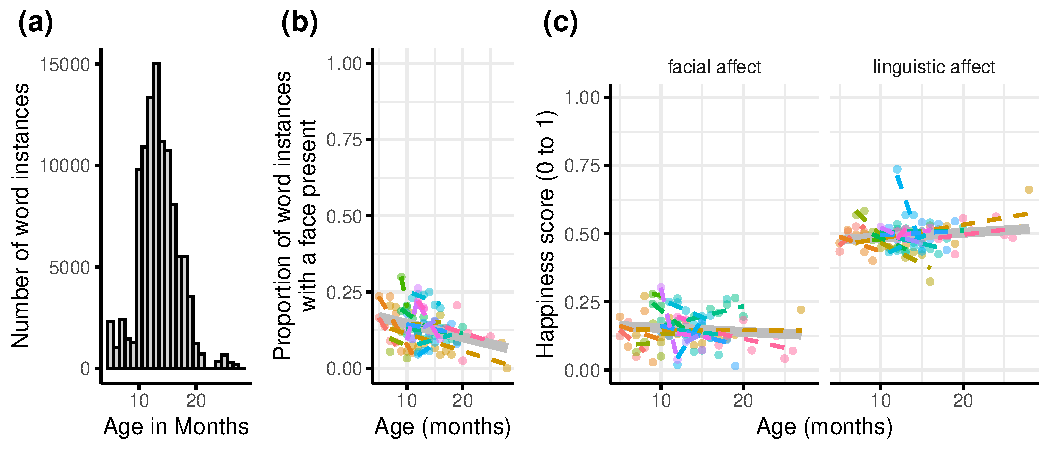
\includegraphics{figs/figure1-1} 

}

\caption[Change in the availability of affective cues with age]{Change in the availability of affective cues with age. (a) Histogram of the word instances across the age range (between 5 and 28 months) in the dataset. (b) Change in the proportion of word instances that coocurred with faces across age. (c) Change in happiness score (from faces - left, or sentiment - right) between the ages of 5 and 28 months. In panels (b-c), the average regression line is plotted in gray. Regression lines for individual participants are plotted with colored dashed lines. Summary data points for each participant (averaged with a single value per participant, per each month of age) are plotted in a color matching the participants’ regression line.}\label{fig:figure1}
\end{figure*}
\end{CodeChunk}

\section{Results}\label{results}

\subsection{Availability of facial and linguistic affect cues across
age}\label{availability-of-facial-and-linguistic-affect-cues-across-age}

How often do infants encounter facial and linguistic affective cues in
the immediate context of early-learned words? On average, 0.1\% of word
instances occurred when a face was in view. This proportion decreased
with age
(\(\beta = -0.04, \textit{t}(15339.4) = -5.96, \textit{p} = < 0.001\);
Figure 1b). Of the word instances where a face was in view concurrently,
the average facial happiness score was 0.16 (out of 1). The happiness
scores for faces coocurring with instances of early-learned words did
not change with age in this dataset
(\(\beta = -9.3e-03, \textit{t}(1349.02) = -0.67, \textit{p} = 0.505\);
Figure 1c - left). Out of all 105,564 word instances, 14,204 (13.46\%)
occurred with a face in view, and 452 (0.43\% of all words and 3.18\% of
all words with a face) of those coocurred with a face that received a
happiness score greater than 0.9.

Linguistic affect was, by definition, more prevalent, because we
measured the affect of the utterances in which words were embedded. Out
of the 105,564 word instances, 29,221 (27.7 \%) were embedded in
utterances that received a sentiment happiness score of 0.9 or higher.
The average sentiment score was 0.47 (out of 1), and, as with facial
affect, this value with not change significantly with age
(\(\beta = 9.3e-03, \textit{t}(2336.48) = 1.42, \textit{p} = 0.156\);
Figure 1c - right).

\begin{CodeChunk}
\begin{figure*}[h]

{\centering 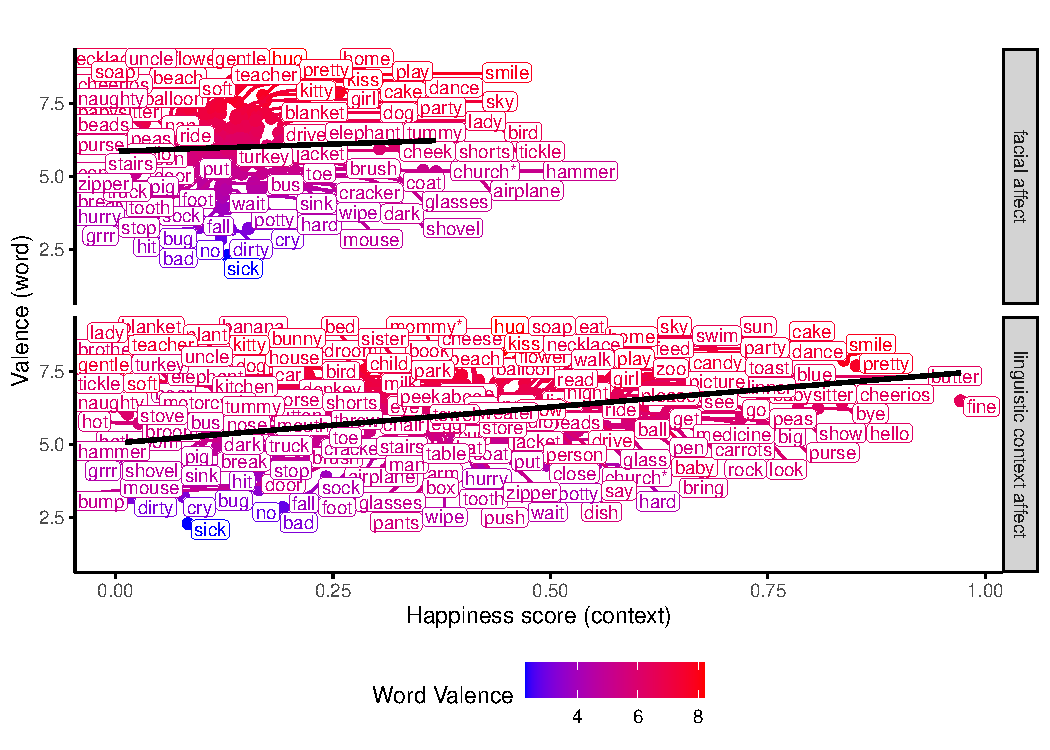
\includegraphics{figs/figure2-1} 

}

\caption[Association between word valence and affective context]{Association between word valence and affective context. The average happiness score (between 0 and 1) for each word of the faces it coocurred with (top panel), and the utterances in which the word was embedded (omitting the word itself; bottom panel). A subset of word labels are visible and colored based on the valence of the word, coded on a scale from 1 (very negative) to 9 (very positive).}\label{fig:figure2}
\end{figure*}
\end{CodeChunk}

\subsection{Words cooccur with matching affective
cues}\label{words-cooccur-with-matching-affective-cues}

Do the affective cues in parents' faces and utterances carry information
about the words they cooccur with? For example, are more positive words
embedded in more positive utterances, and are they more likely to
cooccur with happy faces? We tested these predictions in a mixed effect
model with random intercepts by participant, predicting the valence of
the word from the average facial or linguistic affect it coocurred with
in each video recording, controlling for the frequency of the word. Word
valence was positively associated with the happiness sentiment of the
surrounding utterance
(\(\beta = 0.24, \textit{t}(30490.76) = 43.66, \textit{p} = < 0.001\);
Figure 2 - bottom). For example, the average happiness sentiment score
for the utterances in which the positive word ``smile'' was embedded was
0.84 (out of 1), whereas for the negative word ``cry'' this score was
0.08(out of 1). Similarly, a relatively neutral word like ``eat'' has a
score of 0.47 (out of 1). There were some notable exceptions, like the
word ``gentle,'' which, although positive in valence, appeared in less
positive contexts (e.g., ``I'm worried you need to be a bit more
gentle''). Word valence was less strongly, but still positively
associated with facial happiness (
\(\beta = 0.02, \textit{t}(7197.93) = 2.01, \textit{p} = 0.044\) ;
Figure 2 - top). There was a significant interaction between happiness
score and the modality of the context (faces vs.~sentiment), such that
word valence was more strongly associated with the happiness of the
utterance in which the word was embedded compared to the happiness
displayed by the faces it coocurred with
(\(\beta = 0.21, \textit{t}(37824.69) = 11.3, \textit{p} = < 0.001\)).

\subsection{Sentiment and facial affect do not provide redundant
information}\label{sentiment-and-facial-affect-do-not-provide-redundant-information}

To further probe if the faces and utterances surrounding word instances
carry redundant information, we tested the association between the
average happiness score of the faces vs.~utterances each word coocurred
with. We did so in a mixed effect model where the average happiness
score of each word was predicted by the average happiness score of the
linguistic context (the utterance) in which each word was embedded with
random intercepts by participant. There was no significant association
between facial and linguistic context affect
\(\beta = 8.8e-03, \textit{t}(10367.08) = 0.8, \textit{p} = 0.421\)).

\begin{CodeChunk}
\begin{figure}[H]

{\centering 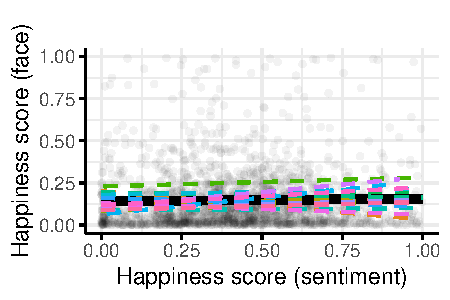
\includegraphics{figs/figure3-1} 

}

\caption[Association between facial and linguistic affect surrounding words]{Association between facial and linguistic affect surrounding words. The average happiness scores for each word, for each recording in the dataset are plotted, with facial affect on the x-axis, and sentiment on the y-axis. The average regression line is plotted in black. Regression lines for individual participants are plotted with colored dashed lines. }\label{fig:figure3}
\end{figure}
\end{CodeChunk}

\section{Discussion}\label{discussion}

The current investigation bridges the gap in our understanding of the
availability of affective cues in the moments when infants encounter
early-learned words in their everyday lives. We found that faces were in
view for only about 1 in 10 words, and an even smaller fraction of those
faces displayed happy affect. Still, more positive words were surrounded
by happier faces. Linguistic context affect (i.e., the utterance in
which a word was embedded), however, conveyed more strongly positive
affect, and was more reliably related to the valence of the word,
compared to facial affect. Together these results suggest that affective
cues in faces and words may have slightly different, but complementary
functions in infants' early learning environments.

The finding that surrounding linguistic context affect can cue the
valence of a word expands prior work showing that the utterances in
which caregivers embed emotion labels like ``happy'' or ``sad'' reflect
the valence of the emotion label (Nencheva et al. (2024)). Although in
this study we did not measure learning, this finding may have
implications about how infants learn valenced words. A consistent
affective context in the utterance surrounding a word can help infants
form connections between similarly valenced words and extract the
meaning of the word with greater ease. Work with older children (from
preschool age to adolescence) shows that children learn valenced
abstract words earlier (Ponari et al. (2020)), and when controlling for
abstractness, children learn positively valenced words earlier (Sabater
et al. (2023)). If the utterances in which these words are embedded
contain information about the valence of these words, this could support
their acquisition, resulting in an earlier age of acquisition. However,
this process requires children to know some positively valenced words to
begin with. What other sources of affective information could infants
use to infer the valence of words, before they build a robust valenced
vocabulary?

Although the proportion of word instances that co-ocurred with faces is
small, it is non-negligible, compared to other impactful learning
signals (e.g., single word-utterances; Braginsky et al. (2016);
Braginsky et al. (2019); Brent \& Siskind (2001); Kosie \& Lew-Williams
(2024); Nencheva et al. (2024); Swingley \& Humphrey (2018)). That is,
faces may be rare, but important. Further, we found evidence that in
those limited instances faces carried information about the valence of
the words they cooccur with. Still, this association was relatively
weak. The lack of a significant association between the affect in the
faces and sentiment suggests that these two signals do not always carry
redundant information in the context of infants' everyday language
experiences. However, although rare in the cases of words and faces,
moments when redundant affective information from different sources is
present may be especially helpful for learning. Such multimodal
redundant affective information has been found to help young infants
discriminate between affective displays (Brady et al. (2024); Flom \&
Bahrick (2007)).

There are several reasons why we may observe a weaker association
between the affect of faces and words (vs.~the affect of target words
and their surrounding linguistic context). One possibility is that our
tools for automatically detecting happiness displays in faces are
imperfect. Face processing tools are relatively newer compared to
language processing tools, and are typically trained on less data (due
to the much higher availability of text data). Although we did a basic
check that the faces that scored highly on happiness indeed represented
happy faces, face processing tools may not be as good at pulling out a
fine-grained gradient score. Another possibility is that canonically
happy faces are an intrinsically noisy signal of positive valence. We do
not always smile when we are trying to convey positive affect. The
significantly lower happiness scores for faces compared to sentiment
suggest that parents are likely conveying positive affect in other ways.
This may be other visual, but more dynamic ways (e.g., through larger
facial movements, or posture changes). An even more important source of
affective information that we did not explore in this investigation is
caregivers' vocal tone. Voices are among the first sources of affective
information available to infants (Grossmann (2010); Haviland \& Lelwica
(1987)), and that the acoustics of caregiver speech have been shown to
convey exaggerated positive affect (Fernald \& Kuhl (1987); Fernald
(1989); Fernald (1992); Kitamura \& Burnham (1998); Singh et al. (2002);
Panneton et al. (2024); Trainor et al. (2000)). A final possibility is
that the affect in faces and words may serve a different function in
early caregiver-child communication. For example, while words may carry
information about the valence of what is talked about, faces may be a
broader socioemotional signal that encourages engagement or bonding.

This investigation comes with several key limitations. First, as
mentioned above, although automated tools allow us to measure affective
information at scale, more work is needed to validate the measurements
provided by these tools and understand how different tools compare to
one another. Second, we focused only on displays of happiness, which do
not reflect the full suite of affective cues available to infants.Third,
it is unclear what temporal window of context is accessible to infants,
and whether more robust information from faces may be available if we
were to expand this window further. In this investigation, we chose to
restrict the analysis window to the duration of the utterance in which
the word was embedded. However, infants may be able to integrate longer
contexts, and the duration of the context from which infants extract
affective information may change depending on their age and the activity
they are engaged in. Fourth, although the dataset we used is a
relatively naturalistic sample of infants' at-home lives, it is still
not a complete representation of infants' experiences. The videos
capture a small sliver of infants' days. Although caregivers were
instructed to capture typical everyday contexts, they may still be more
likely to attempt a video recording when their child is in a neutral or
positive mood, to avoid fussiness around wearing the camera helmet.
Caregivers may also be especially motivated to interact with their child
when being recorded. Further, the data used were not uniformly
distributed across the age range, making it challenging to estimate how
the availability of these cues change with age. Finally, we only focused
on two of the many sources of affective information accessible to
infants, and we did not differentiate between the sources of these cues.
For example, the faces infants observed included faces from caregivers
as well as siblings. How infants integrate affective information from
these different sources is unknown.

The current investigation underscores the importance of characterizing
the emotional contexts surrounding early language input in infants'
natural learning environments. By examining how facial and linguistic
cues align---or fail to align---with the valence of words, this
investigation highlights the unique roles these cues may play in shaping
infants' word learning. Such findings emphasize the need to move beyond
controlled, laboratory-based studies to capture the complexities of
real-world experience. Ultimately, this research contributes to a
growing body of evidence that infants' early language experiences are
deeply embedded in multimodal and affect-rich environments, which are
crucial for supporting their development and learning.

\section{Acknowledgements}\label{acknowledgements}

{[}omitted for blind review{]}

\section{References}\label{references}

\setlength{\parindent}{-0.1in} 
\setlength{\leftskip}{0.125in}

\noindent

\phantomsection\label{refs}
\begin{CSLReferences}{1}{0}
\bibitem[\citeproctext]{ref-andrews2009integrating}
Andrews, M., Vigliocco, G., \& Vinson, D. (2009). Integrating
experiential and distributional data to learn semantic representations.
\emph{Psychological Review}, \emph{116}(3), 463.

\bibitem[\citeproctext]{ref-lme4}
Bates, D., Mächler, M., Bolker, B., \& Walker, S. (2015). Fitting linear
mixed-effects models using {lme4}. \emph{Journal of Statistical
Software}, \emph{67}(1), 1--48.
\url{https://doi.org/10.18637/jss.v067.i01}

\bibitem[\citeproctext]{ref-benders2013mommy}
Benders, T. (2013). Mommy is only happy! Dutch mothers' realisation of
speech sounds in infant-directed speech expresses emotion, not didactic
intent. \emph{Infant Behavior and Development}, \emph{36}(4), 847--862.

\bibitem[\citeproctext]{ref-bergelson2016bergelson}
Bergelson, E. (2016). Bergelson seedlings homebank corpus. \emph{Doi},
\emph{10}, T5PK6D.

\bibitem[\citeproctext]{ref-bergelson2019day}
Bergelson, E., Amatuni, A., Dailey, S., Koorathota, S., \& Tor, S.
(2019). Day by day, hour by hour: Naturalistic language input to
infants. \emph{Developmental Science}, \emph{22}(1), e12715.

\bibitem[\citeproctext]{ref-brady2024effects}
Brady, S. M., Ogren, M., \& Johnson, S. P. (2024). Effects of
conflicting emotional cues on toddlers' emotion perception.
\emph{British Journal of Developmental Psychology}.

\bibitem[\citeproctext]{ref-braginsky2016uh}
Braginsky, M., Yurovsky, D., Marchman, V. A., \& Frank, M. (2016). From
uh-oh to tomorrow: Predicting age of acquisition for early words across
languages. \emph{CogSci}, \emph{6}.

\bibitem[\citeproctext]{ref-braginsky2019consistency}
Braginsky, M., Yurovsky, D., Marchman, V. A., \& Frank, M. C. (2019).
Consistency and variability in children's word learning across
languages. \emph{Open Mind}, \emph{3}, 52--67.

\bibitem[\citeproctext]{ref-brent2001role}
Brent, M. R., \& Siskind, J. M. (2001). The role of exposure to isolated
words in early vocabulary development. \emph{Cognition}, \emph{81}(2),
B33--B44.

\bibitem[\citeproctext]{ref-cheong2023py}
Cheong, J. H., Jolly, E., Xie, T., Byrne, S., Kenney, M., \& Chang, L.
J. (2023). Py-feat: Python facial expression analysis toolbox.
\emph{Affective Science}, \emph{4}(4), 781--796.

\bibitem[\citeproctext]{ref-feng2024child}
Feng, S. Y., Goodman, N. D., \& Frank, M. C. (2024). Is child-directed
speech effective training data for language models? \emph{arXiv Preprint
arXiv:2408.03617}.

\bibitem[\citeproctext]{ref-fernald1989intonation}
Fernald, A. (1989). Intonation and communicative intent in mothers'
speech to infants: Is the melody the message? \emph{Child Development},
1497--1510.

\bibitem[\citeproctext]{ref-fernald1992human}
Fernald, A. (1992). Human maternal vocalizations to in-fants as
biologically relevant signals {[}{]}. \emph{The Adapted Mind:
Evolu-Tionary Psychology and the Generation of Culture}.

\bibitem[\citeproctext]{ref-fernald1987acoustic}
Fernald, A., \& Kuhl, P. (1987). Acoustic determinants of infant
preference for motherese speech. \emph{Infant Behavior and Development},
\emph{10}(3), 279--293.

\bibitem[\citeproctext]{ref-flom2007development}
Flom, R., \& Bahrick, L. E. (2007). The development of infant
discrimination of affect in multimodal and unimodal stimulation: The
role of intersensory redundancy. \emph{Developmental Psychology},
\emph{43}(1), 238.

\bibitem[\citeproctext]{ref-goldstein2008social}
Goldstein, M. H., \& Schwade, J. A. (2008). Social feedback to infants'
babbling facilitates rapid phonological learning. \emph{Psychological
Science}, \emph{19}(5), 515--523.

\bibitem[\citeproctext]{ref-grossmann2010development}
Grossmann, T. (2010). The development of emotion perception in face and
voice during infancy. \emph{Restorative Neurology and Neuroscience},
\emph{28}(2), 219--236.

\bibitem[\citeproctext]{ref-haviland1987induced}
Haviland, J. M., \& Lelwica, M. (1987). The induced affect response:
10-week-old infants' responses to three emotion expressions.
\emph{Developmental Psychology}, \emph{23}(1), 97.

\bibitem[\citeproctext]{ref-hennessy2023building}
Hennessy, V., \& Zhao, T. C. (2023). \emph{Building the bond: The
social-emotional role of infant-directed speech \& song}.

\bibitem[\citeproctext]{ref-kim2013young}
Kim, H. I., \& Johnson, S. P. (2013). Do young infants prefer an
infant-directed face or a happy face? \emph{International Journal of
Behavioral Development}, \emph{37}(2), 125--130.

\bibitem[\citeproctext]{ref-kitamura1998infant}
Kitamura, C., \& Burnham, D. (1998). The infant's response to maternal
vocal affect. \emph{Advances in Infancy Research}, \emph{12}, 221--236.

\bibitem[\citeproctext]{ref-kosie2024infant}
Kosie, J. E., \& Lew-Williams, C. (2024). Infant-directed communication:
Examining the many dimensions of everyday caregiver-infant interactions.
\emph{Developmental Science}, \emph{27}(5), e13515.

\bibitem[\citeproctext]{ref-kusal2023systematic}
Kusal, S., Patil, S., Choudrie, J., Kotecha, K., Vora, D., \& Pappas, I.
(2023). A systematic review of applications of natural language
processing and future challenges with special emphasis in text-based
emotion detection. \emph{Artificial Intelligence Review}, \emph{56}(12),
15129--15215.

\bibitem[\citeproctext]{ref-lmerTest}
Kuznetsova, A., Brockhoff, P. B., \& Christensen, R. H. B. (2017).
{lmerTest} package: Tests in linear mixed effects models. \emph{Journal
of Statistical Software}, \emph{82}(13), 1--26.
\url{https://doi.org/10.18637/jss.v082.i13}

\bibitem[\citeproctext]{ref-leong2023facial}
Leong, S. C., Tang, Y. M., Lai, C. H., \& Lee, C. (2023). Facial
expression and body gesture emotion recognition: A systematic review on
the use of visual data in affective computing. \emph{Computer Science
Review}, \emph{48}, 100545.

\bibitem[\citeproctext]{ref-LoBue2024}
LoBue, V., Ogrent, M., Leottit, L., Hoemann, K., Oakes, L. M., \&
Barrett, L. F. (2024). \emph{Describing the emotional environment of the
infant}.

\bibitem[\citeproctext]{ref-long2022longitudinal}
Long, B. L., Kachergis, G., Agrawal, K., \& Frank, M. C. (2022). A
longitudinal analysis of the social information in infants' naturalistic
visual experience using automated detections. \emph{Developmental
Psychology}, \emph{58}(12), 2211.

\bibitem[\citeproctext]{ref-long2022automated}
Long, B. L., Sanchez, A., Kraus, A. M., Agrawal, K., \& Frank, M. C.
(2022). Automated detections reveal the social information in the
changing infant view. \emph{Child Development}, \emph{93}(1), 101--116.

\bibitem[\citeproctext]{ref-long2024babyview}
Long, B., Xiang, V., Stojanov, S., Sparks, R. Z., Yin, Z., Keene, G. E.,
Tan, A. W., Feng, S. Y., Zhuang, C., Marchman, V. A., et al. (2024). The
BabyView dataset: High-resolution egocentric videos of infants' and
young children's everyday experiences. \emph{arXiv Preprint
arXiv:2406.10447}.

\bibitem[\citeproctext]{ref-morgan2023mother}
Morgan, J. K., Santosa, H., Conner, K. K., Fridley, R. M., Forbes, E.
E., Iyengar, S., Joseph, H. M., \& Huppert, T. J. (2023). Mother--child
neural synchronization is time linked to mother--child positive
affective state matching. \emph{Social Cognitive and Affective
Neuroscience}, \emph{18}(1), nsad001.

\bibitem[\citeproctext]{ref-nencheva2024word}
Nencheva, M. L., Schwab, J. F., Lew-Williams, C., \& Fausey, C. M.
(2024). Word repetition and isolation are intertwined in children's
early language experiences. \emph{Open Mind}, \emph{8}, 1330--1347.

\bibitem[\citeproctext]{ref-nencheva2023caregiver}
Nencheva, M. L., Tamir, D. I., \& Lew-Williams, C. (2023). Caregiver
speech predicts the emergence of children's emotion vocabulary.
\emph{Child Development}, \emph{94}(3), 585--602.

\bibitem[\citeproctext]{ref-nguyen2024visualizing}
Nguyen, T., Kungl, M. T., Hoehl, S., White, L. O., \& Vrtička, P.
(2024). Visualizing the invisible tie: Linking parent--child neural
synchrony to parents' and children's attachment representations.
\emph{Developmental Science}, \emph{27}(6), e13504.

\bibitem[\citeproctext]{ref-Ogren2024}
Ogren, M., Leottit, L., Hoemann, K., Oakes, L. M., Barrett, L. F., \&
LoBue, V. (2024). \emph{The early emotional environment: What facial
configurations do infants typically see in natural social interactions?}

\bibitem[\citeproctext]{ref-orhan2024learning}
Orhan, A. E., \& Lake, B. M. (2024). Learning high-level visual
representations from a child's perspective without strong inductive
biases. \emph{Nature Machine Intelligence}, \emph{6}(3), 271--283.

\bibitem[\citeproctext]{ref-panneton2024positive}
Panneton, R., Cristia, A., Taylor, C., \& Christine, M. (2024). Positive
valence contributes to hyperarticulation in maternal speech to infants
and puppies. \emph{Journal of Child Language}, \emph{51}(5), 1230--1240.

\bibitem[\citeproctext]{ref-panneton2006slow}
Panneton, R., Kitamura, C., Mattock, K., \& Burnham, D. (2006). Slow
speech enhances younger but not older infants' perception of vocal
emotion. \emph{Research in Human Development}, \emph{3}(1), 7--19.

\bibitem[\citeproctext]{ref-ponari2018acquisition}
Ponari, M., Norbury, C. F., \& Vigliocco, G. (2018). Acquisition of
abstract concepts is influenced by emotional valence.
\emph{Developmental Science}, \emph{21}(2), e12549.

\bibitem[\citeproctext]{ref-ponari2020role}
Ponari, M., Norbury, C. F., \& Vigliocco, G. (2020). The role of
emotional valence in learning novel abstract concepts.
\emph{Developmental Psychology}, \emph{56}(10), 1855.

\bibitem[\citeproctext]{ref-sabater2023acquisition}
Sabater, L., Ponari, M., Haro, J., Fernández-Folgueiras, U., Moreno, E.
M., Pozo, M. A., Ferré, P., \& Hinojosa, J. A. (2023). The acquisition
of emotion-laden words from childhood to adolescence. \emph{Current
Psychology}, \emph{42}(33), 29280--29290.

\bibitem[\citeproctext]{ref-Savani2024}
Savani, B. (2024). \emph{Bert-base-uncased-emotion {[}pretrained
model{]}}. Hugging Face.
\url{https://huggingface.co/bhadresh-savani/bert-base-uncased-emotion}

\bibitem[\citeproctext]{ref-singh2002infants}
Singh, L., Morgan, J. L., \& Best, C. T. (2002). Infants' listening
preferences: Baby talk or happy talk? \emph{Infancy}, \emph{3}(3),
365--394.

\bibitem[\citeproctext]{ref-sullivan2021saycam}
Sullivan, J., Mei, M., Perfors, A., Wojcik, E., \& Frank, M. C. (2021).
SAYCam: A large, longitudinal audiovisual dataset recorded from the
infant's perspective. \emph{Open Mind}, \emph{5}, 20--29.

\bibitem[\citeproctext]{ref-swingley2018quantitative}
Swingley, D., \& Humphrey, C. (2018). Quantitative linguistic predictors
of infants' learning of specific english words. \emph{Child
Development}, \emph{89}(4), 1247--1267.

\bibitem[\citeproctext]{ref-trainor2000infant}
Trainor, L. J., Austin, C. M., \& Desjardins, R. N. (2000). Is
infant-directed speech prosody a result of the vocal expression of
emotion? \emph{Psychological Science}, \emph{11}(3), 188--195.

\bibitem[\citeproctext]{ref-warstadt2023findings}
Warstadt, A., Mueller, A., Choshen, L., Wilcox, E., Zhuang, C., Ciro,
J., Mosquera, R., Paranjabe, B., Williams, A., Linzen, T., et al.
(2023). Findings of the BabyLM challenge: Sample-efficient pretraining
on developmentally plausible corpora. \emph{Proceedings of the BabyLM
Challenge at the 27th Conference on Computational Natural Language
Learning}.

\bibitem[\citeproctext]{ref-zieber2014infants}
Zieber, N., Kangas, A., Hock, A., \& Bhatt, R. S. (2014). Infants'
perception of emotion from body movements. \emph{Child Development},
\emph{85}(2), 675--684.

\end{CSLReferences}

\bibliographystyle{apacite}


\end{document}
